\chapter{結果}
\label{ch:results}
\ref{ch:results}章では、\ref{ch:mm_analysis}章で紹介した手法を踏まえて導出した柱密度の結果について述べていく。
まず、トロムソと昭和基地で共通してわかったこととしては、どちらとも\ce{NO}の短期的変動が確認できたことである。
以降、トロムソ(\ref{sec:results_tromsoe}節)と昭和基地(\ref{sec:results_syowa}節)と観測場所別に分けて述べていく。

\section{ノルウェー・トロムソでの解析結果}
\label{sec:results_tromsoe}
スクリーニングの結果、2つの期間が残った。
1つ目の期間は、2019年1月23日〜2019年2月4日、2つ目の期間は2019年2月17日〜2019年2月20日となった。
参考として2つの期間の間の時間変動を確認するため、本来スクリーニングされた期間(2019年2月5日〜2019年2月16日)についてもプロットした(図\ref{fig:avg_ColumnDensity_tromsoe}のグレーのエラーバー)。
時間分解能は24時間となり、プロット間隔も24時間(1日1プロット)とした。
\begin{figure}[htbp]
    \centering
    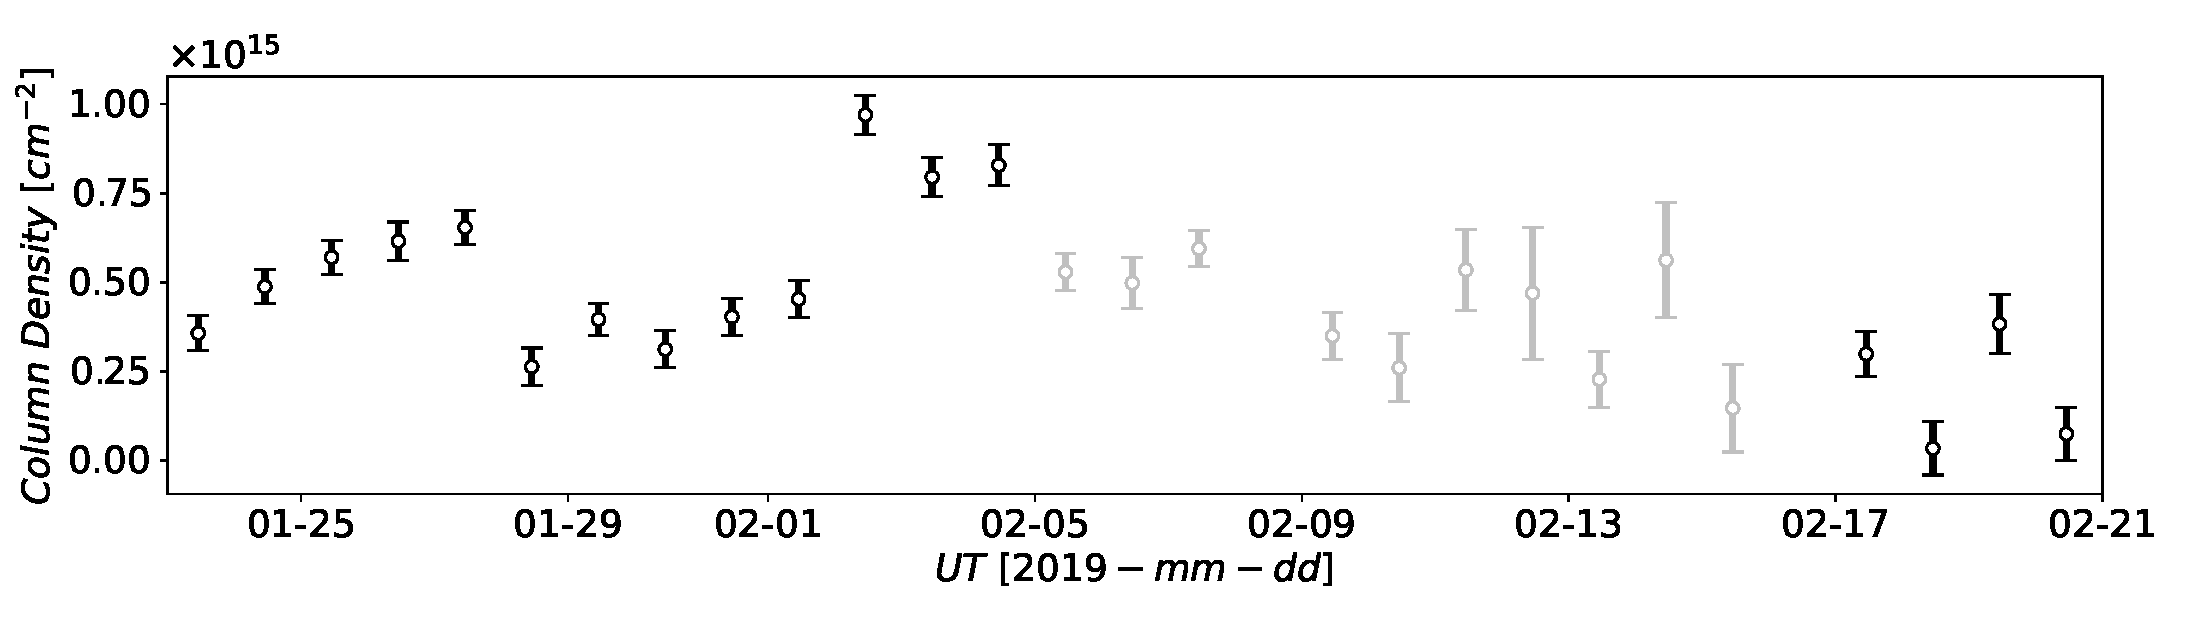
\includegraphics[width=\linewidth]{master_thesis_contents/master_thesis_fig/avg_ColumnDensity_tromsoe.pdf}
    \caption{トロムソにおける\ce{NO}柱密度の時間変動(グレーのエラーバーは本来スクリーニングされた期間であることを示す)}
    \label{fig:avg_ColumnDensity_tromsoe}
\end{figure}
\ce{NO}の柱密度について、エラーバーの範囲を超える有意な増加がみられる期間が2つあった(2019年1月23日〜2019年1月27日と2019年2月1日〜2019年2月4日)。
1つ目の時期(2019年1月23日〜2019年1月27日)16\% の緩やかな増加となり、2つ目の時期(2019年2月1日〜2019年2月4日)は83\% の急激な増加が確認できた。


\section{南極・昭和基地での解析結果}
\label{sec:results_syowa}
スクリーニングの結果、2023年3月22日〜2023年3月30日の期間が残った。
昭和基地ではNOの6本の超微細構造線を全て用いることで、積分時間は12時間とし、プロット間隔は6時間とした。
その結果、柱密度の誤差の平均は、積分時間が24時間であるトロムソの解析結果(\ref{sec:results_tromsoe}節の図\ref{fig:avg_ColumnDensity_tromsoe})と比べて20\% 小さくすることができ、時間分解能は12時間と良くなった。
\ce{NO}の柱密度について、エラーバーの範囲を超える有意な増加がみられる期間が2つあった(2023年3月23日21時〜2023年3月24日3時と2023年3月25日9時〜2023年3月25日21時)。
どちらも1プロットごとに増加となった。
\begin{figure}[htbp]
    \centering
    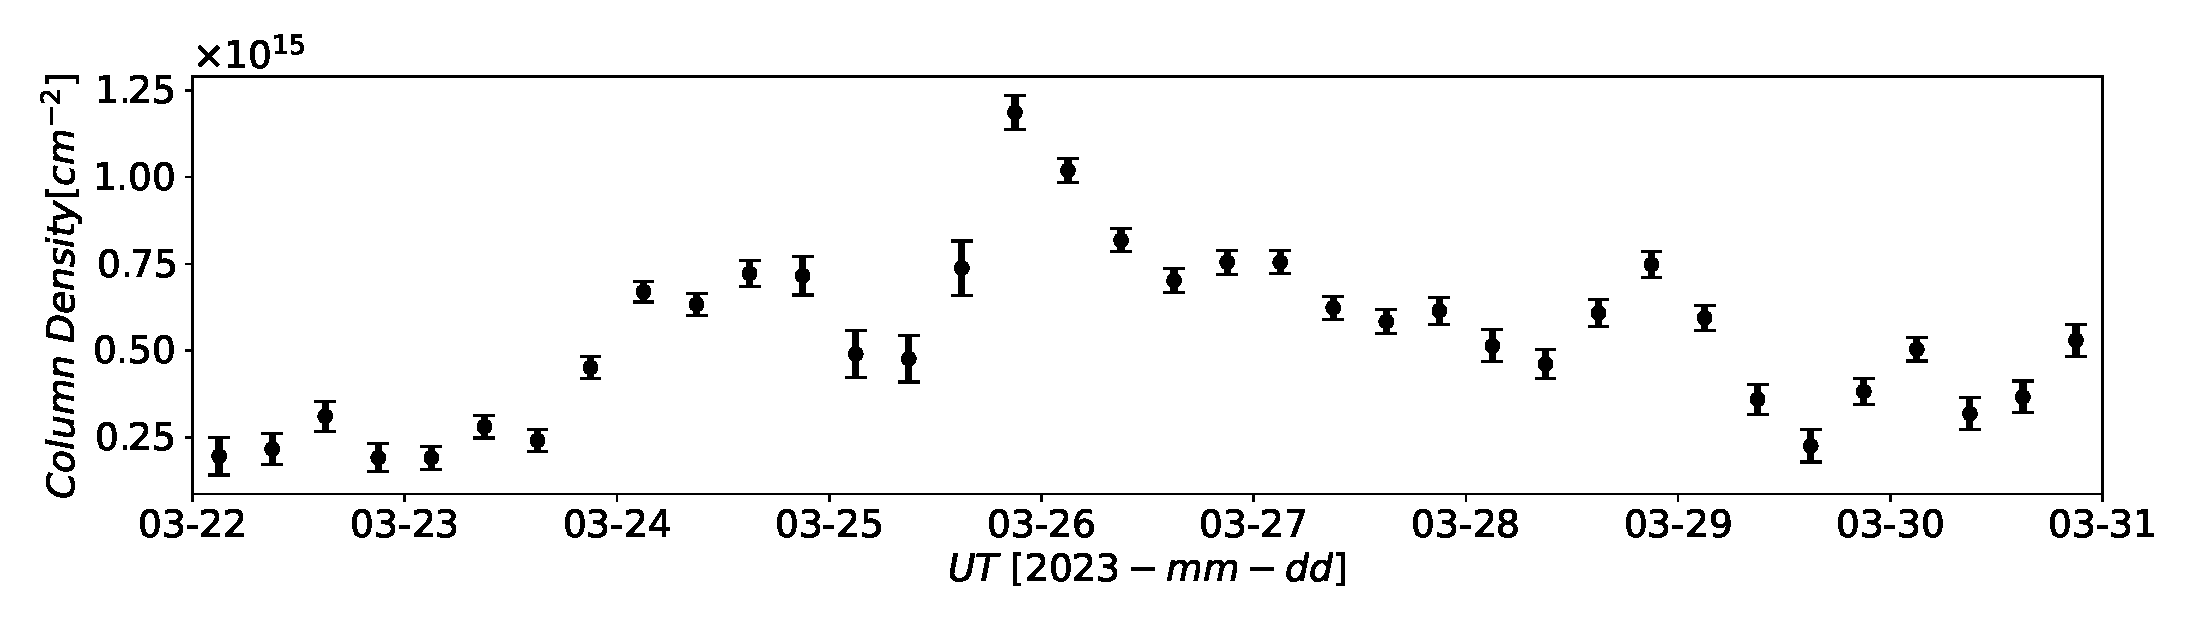
\includegraphics[width=\linewidth]{master_thesis_contents/master_thesis_fig/column_density_spectr6_syowa.pdf}
    \caption{昭和基地における\ce{NO}柱密度の時間変動}
    \label{fig:column_density_spectr6_syowa}
\end{figure}
